\section{BACKGROUND}
\subsection{Project Context}
The [Project Name] project aimed to support BVI participants in developing video creation skills they could continue using in their own creative practice beyond the workshop series. Between April and July 2025 we ran seven structured workshops co-designed and co-delivered with three UK BVI-sector partner organisations (two in [City 1], one in [City 2]), here anonymised as [Partner A], [Partner B], and [Partner C]. The partners supported recruitment, co-facilitation, and integration of the workshops within existing community programmes.

\subsection{Workshop Structure and Curriculum}
Each workshop ran 3--4 hours and followed a consistent session structure. Sessions opened with a brief warm-up that included introductions with visual descriptions, the day's aims, and an outline of activities. Core teaching combined short demonstrations with hands-on practice; in-person sessions had a teaching team of two tutors and one facilitator who circulated to support participants individually, while online sessions were tutor-led with support provided remotely. Sessions closed with a 20--30-minute facilitated reflection focused on challenges, accessibility, and next steps (rationale and procedure in \autoref{sec:design-rationale}). Each workshop was supported by accessible workbooks providing step-by-step VoiceOver-compatible instructions and by teaching slides adapted for screen-reader compatibility.

\begin{figure}
    \centering
    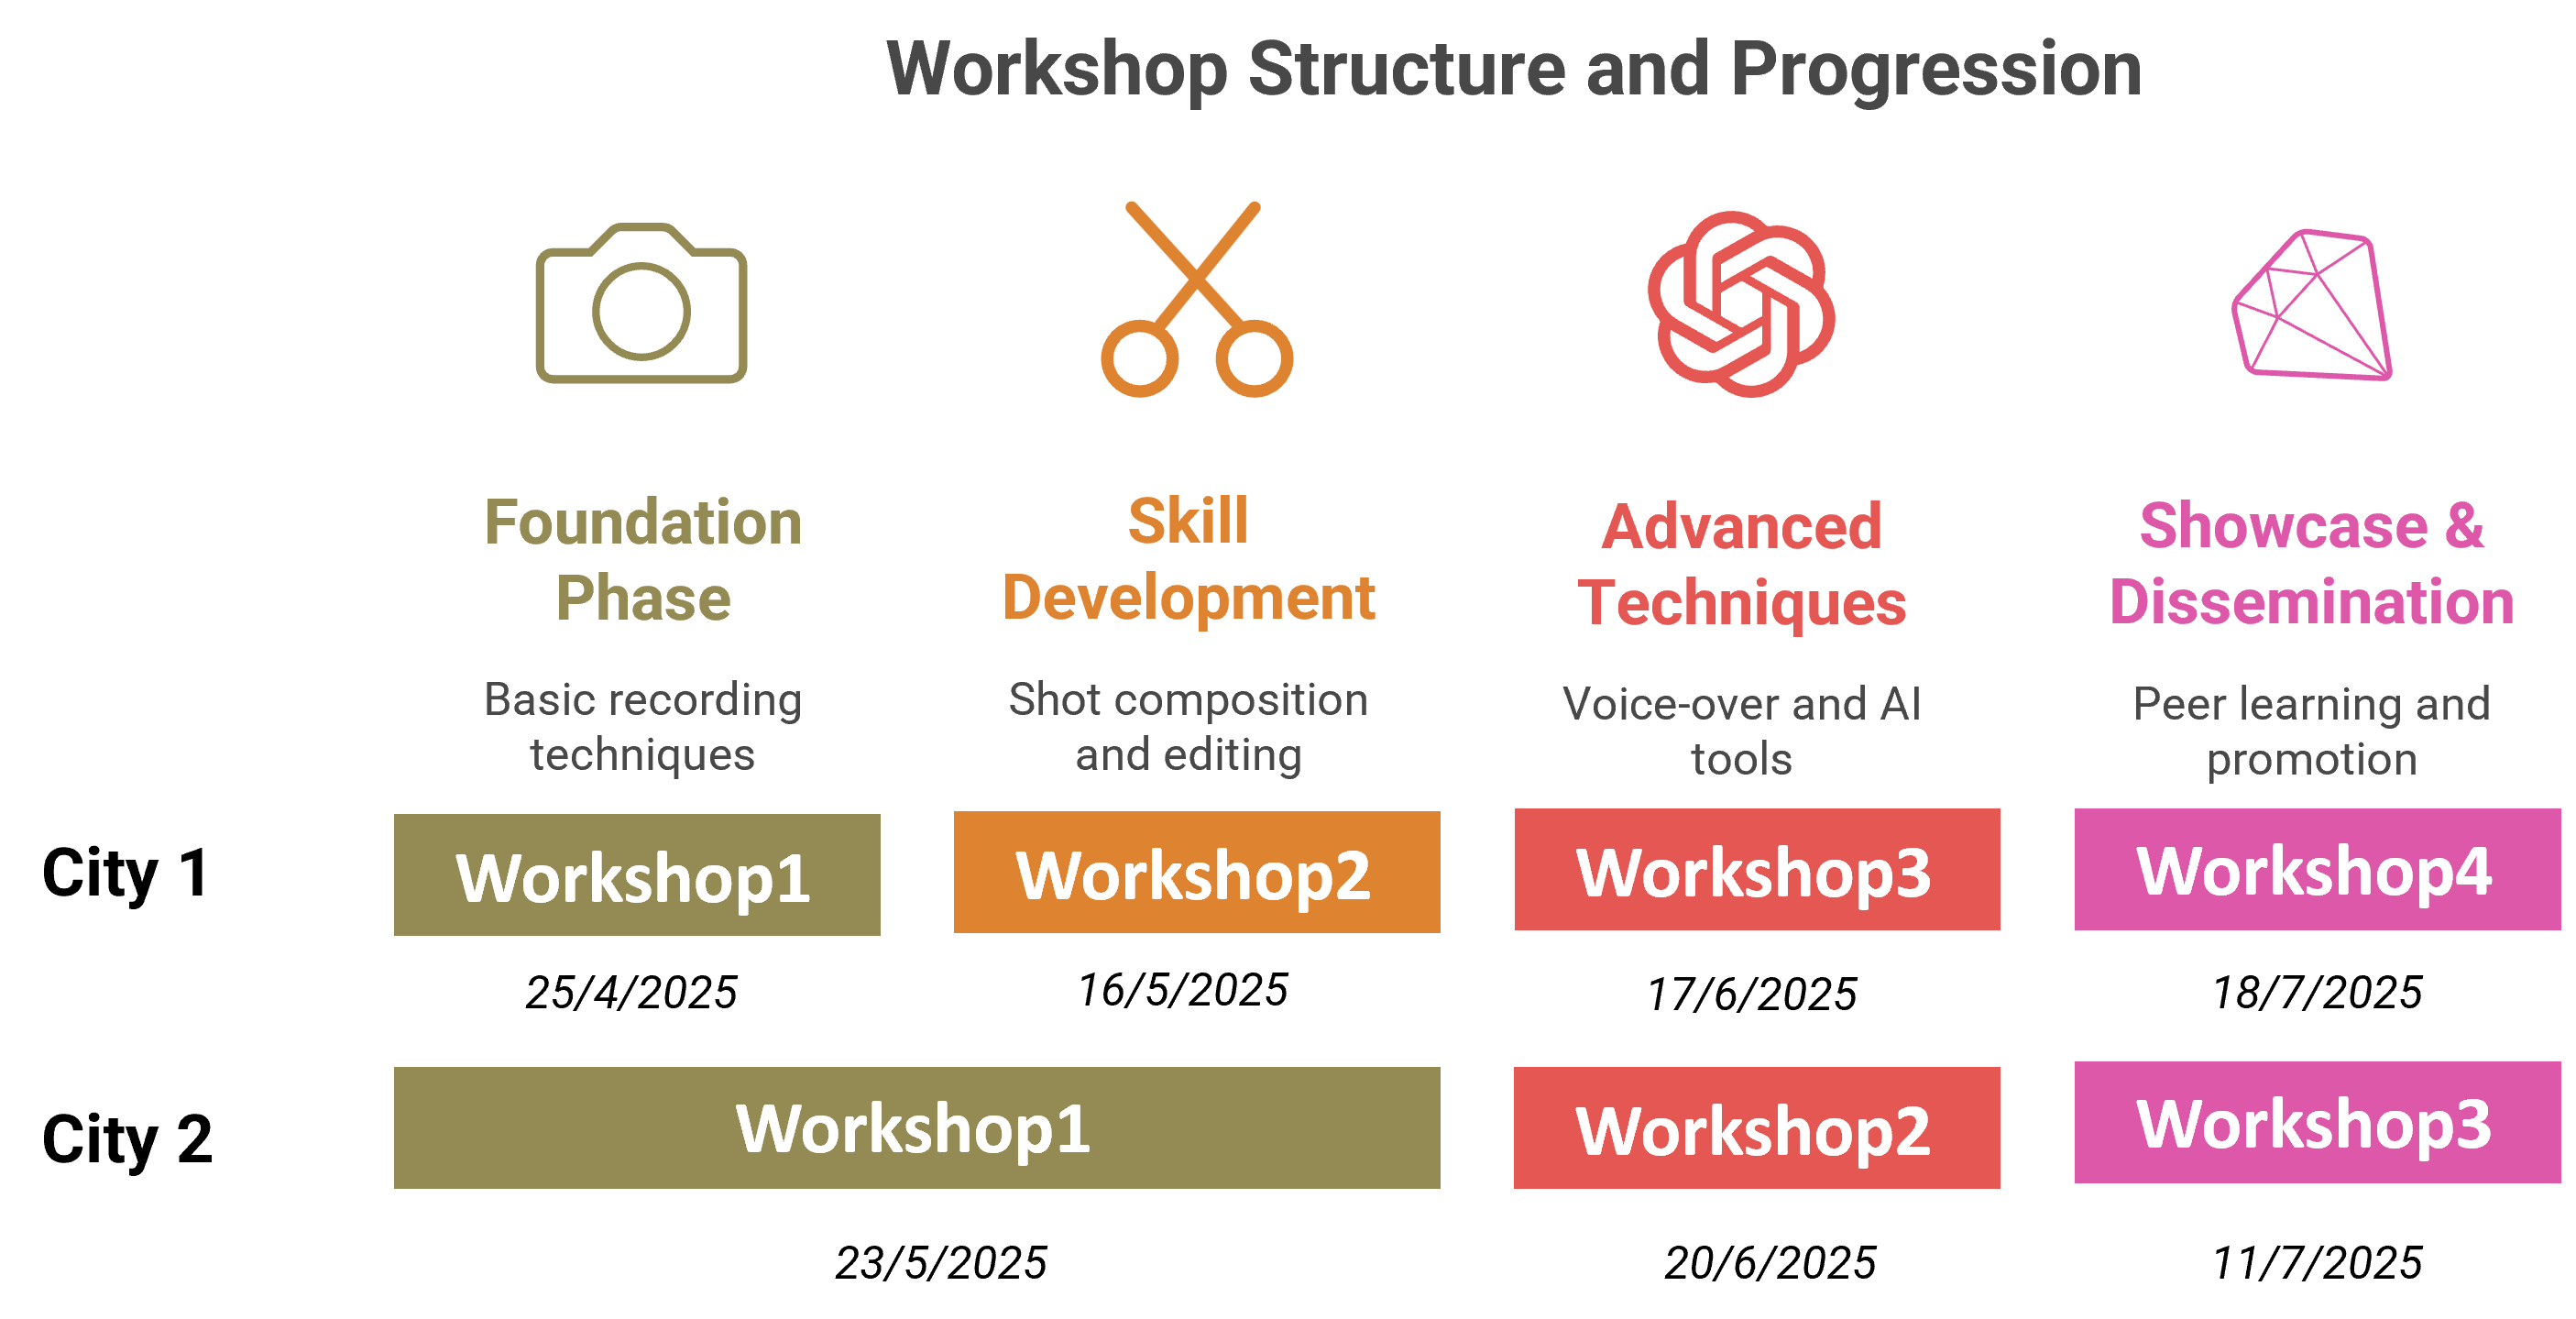
\includegraphics[width=1\linewidth]{Pics/workshop_am.png}
    \caption{Infographic of the four-phase curriculum: Foundation, Skill Development, Advanced Techniques, and Showcase \& Dissemination, with color-coded columns and rows mapping the [City 1] (Workshops 1--4) and [City 2] (Workshops 1--3) sequences.}
    \label{fig:workshop}
    \Description{Infographic with four columns that label the curriculum phases: Foundation Phase (basic recording techniques), Skill Development (shot composition and editing), Advanced Techniques (voice-over and AI tools), and Showcase \& Dissemination (peer learning and promotion). A top row of boxes maps one workshop to each phase for the [City 1] site (Workshops 1-4). A second row shows the [City 2] site configuration where Foundation and Skill Development are combined into Workshop 1, Advanced Techniques is Workshop 2, and Showcase \& Dissemination is Workshop 3.}
\end{figure}

The curriculum followed a scaffolded path (see \autoref{fig:workshop}). The Foundation phase oriented participants to accessible apps and basic equipment (ring lights, tripods, microphones) and covered fundamentals of audio and video capture, with emphasis on confidence in camera pointing, framing through non-visual feedback, and creating simple recordings with music. The Skill-Development phase introduced shot composition (close and wide shots), trimming, basic editing, and music integration, with Seeing AI used as a key tool for framing and recording by providing real-time audio feedback about visual composition. The Advanced Techniques phase covered voice-over narration and AI-assisted graphic generation (stylised selfies, logos, text assets) to extend creative options. The Showcase \& Dissemination phase centred on peer sharing of works-in-progress, advanced prompting strategies, and approaches to online sharing and promotion. Phase-to-workshop mapping differed across the two sites for reasons described in \autoref{sec:design-rationale}.

\subsection{Participants and Teaching Team}

\begin{table}[]
\begin{tabular}{@{}ccccc@{}}
\toprule
\textbf{ID} & \textbf{Age Group} & \textbf{Gender} & \textbf{Vision Profile} & \textbf{Media Creation Experience (0--5)} \\ \midrule
P1          & 40--65              & Female          & Low Vision              & 2                                        \\
P2          & 40--65              & Female          & Low Vision              & 1                                        \\
P3          & 40--65              & Female          & Low Vision              & 2                                        \\
P4          & Over 65            & Male            & Blind                   & 1                                        \\
P5          & 26--39              & Female          & Low Vision              & 3                                        \\
P6          & 40--65              & Female          & Blind                   & 1                                        \\
P7          & 26--39              & Male            & Blind                   & 2                                        \\
P8          & 26--39              & Female          & Blind                   & 1                                        \\
P9          & 26--39              & Female          & Low Vision              & 1                                        \\
P10         & 40--65              & Female          & Blind                   & 1                                        \\
T1          & 26--39              & Male            & Sighted                 & 5                                        \\
T2          & 26--39              & Male            & Sighted                 & 3                                        \\
T3          & 26--39              & Female          & Low Vision              & 4                                        \\
T4          & 26--39              & Female          & Blind                   & 4                                        \\ \bottomrule
\end{tabular}
\caption{Demographics of participants and teaching team. P denotes participant, T denotes teaching team.}
\label{tab:demo}
\end{table}

We engaged 13 BVI participants across two cohorts; three withdrew during the series due to scheduling conflicts or health-related reasons and are not included in the analysis. Recruitment used purposive sampling through partner networks to support diversity in vision conditions, technology experience, and creative backgrounds. Inclusion criteria were self-identification as blind or visually impaired and basic smartphone familiarity; prior video experience was not required. The analytic sample comprises 10 participants (\autoref{tab:demo}; IDs use P for participants and T for teaching team): 8 women and 2 men; ages 26--39 (n=4), 40--65 (n=5), and over 65 (n=1). Vision profiles were evenly split between low vision (n=5) and blind (n=5). Self-rated media-creation experience on a 0--5 scale averaged 1.5 (median 1, range 1--3). Two participants (P3, P4) attended with sighted helpers (\autoref{sec:design-rationale}).

The facilitation team comprised four members in the 26--39 age range with gender balance (two women, two men) and substantial media-creation experience (mean 4.0, range 3--5): a sighted lead tutor (T1), two BVI tutors with video expertise (one low vision (T3), one blind (T4)), and one sighted facilitator providing technical support and visual description (T2). Two team members were drawn from the research team and two were tutor-assistant-trainees nominated by the partner organisations from the [City 1] and [City 2] communities, supporting capacity building within the BVI community.

\paragraph{Sighted helpers.}
Two participants (P3, P4) attended with sighted helpers across the workshops. Helpers were paid support workers or family members. None received role briefing or VoiceOver orientation before the sessions; their digital competence and prior familiarity with the participant varied, and this variation shaped several of the episodes documented in \autoref{sec:results} (see also \autoref{sec:limitations}). Typical helper contributions included device positioning, menu reading, informal coaching, and occasional substitution on visual-verification tasks. We documented helper--participant interactions through field notes and, where helpers consented, through video recording; no formal helper interviews were conducted, for the reasons given in \autoref{sec:design-rationale}. We therefore describe helpers' actions in \autoref{sec:results} as observed rather than as self-reported.
